\documentclass[conference]{IEEEtran}
\IEEEoverridecommandlockouts
\usepackage{cite}
\usepackage{amsmath,amssymb,amsfonts}
\usepackage{graphicx}
\usepackage{textcomp}
% Tectonic/XeTeX uses TU encoding, where IEEEtran's requested Times (ptm) and
% Courier (pcr) shapes are undefined -- bold silently degrades to medium.
% newtx supplies Times-compatible text and math with correct bold shapes.
\usepackage{newtxtext,newtxmath}
\usepackage{xcolor}
\usepackage{booktabs}
\usepackage{array}
\newcolumntype{L}[1]{>{\raggedright\arraybackslash}p{#1}}
\usepackage[ruled,vlined]{algorithm2e}
\usepackage{rotating}
\graphicspath{{figures/}}

\begin{document}

\title{A Hybrid Multi-Stage Deep Learning Model for\\
River Water Quality Prediction and\\
Pollution Anomaly Detection}

\author{
\IEEEauthorblockN{Raghav Subramaniam, S. Tejas Karthikeyan, Nithyasree Ganesan}
\IEEEauthorblockA{Department of Information Science and Technology\\
College of Engineering Guindy, Anna University\\
Chennai 600025, India}
}

\maketitle

\begin{abstract}
Water quality time series are nonlinear, nonstationary and irregularly sampled,
which limits conventional forecasting methods. This paper presents a hybrid
framework coupling Complete Ensemble Empirical Mode Decomposition with
Adaptive Noise (CEEMDAN) with a convolutional--recurrent network and a
self-attention layer. Nine measured parameters are each decomposed into
intrinsic mode functions, giving an 81-channel input passed through a 1-D CNN,
an LSTM and attention pooling to jointly predict all nine. A per-parameter
residual baseline additionally drives a $3\sigma$ anomaly detector. On 1{,}085
observations spanning 2016--2024, the model reduces mean absolute error against
a persistence baseline on seven of nine parameters, by up to 33\%. The point
accuracy initially targeted was not attained, with coefficients of
determination remaining near or below zero. Decomposing this result, however,
shows it stems from amplitude damping rather than from a failure to learn
temporal structure. For the
seasonally driven parameters the prediction tracks the observed series in
correct phase (Pearson $r=0.56$ for temperature, $0.48$ for dissolved oxygen)
while reproducing only 65--73\% of its variance. The temporal stream recovers
\emph{when} parameters move but not \emph{how far}. We argue the missing
amplitude information is largely spatial, and that the natural next step is to
pair this temporal expert with a spatial expert over remotely sensed catchment
features under a learned fusion gate.
\end{abstract}

\begin{IEEEkeywords}
Water quality prediction, CEEMDAN, CNN, LSTM, self-attention, anomaly
detection, sensor fusion
\end{IEEEkeywords}

\section{Introduction}

\subsection{Background and Motivation}

Water quality refers to the chemical, physical and biological characteristics
that determine a water body's suitability for drinking, irrigation, industry or
aquatic life. It directly influences biodiversity, agricultural productivity and
public health, yet industrialisation and urbanisation have made contamination by
nutrients, heavy metals and organic pollutants a pressing global concern.
Accurate prediction of water quality parameters is therefore central to early
pollution warning and sustainable resource planning.

Routine monitoring centres on a small set of indicators. \emph{Dissolved
oxygen} governs the survival of aquatic organisms, with depressed levels
producing fish kills; \emph{pH} controls metal solubility and biological
function; \emph{turbidity} measures suspended particulate load and limits light
penetration; and \emph{conductivity} and \emph{total dissolved solids} track
the ionic content that indicates industrial or saline intrusion. Nutrient
species -- ammonia, nitrates and phosphates -- drive eutrophication. This work
predicts all nine such parameters jointly.

Prediction is difficult for reasons intrinsic to the data. Measurements are \emph{nonlinear}, since parameters interact through
coupled biochemical processes: a rise in temperature depresses dissolved oxygen
saturation, while nutrient loading drives algal activity that perturbs both.
They are \emph{nonstationary}, as seasonal cycles and land-use change shift the
underlying distribution. They are \emph{noisy}, and \emph{sparsely sampled},
since routine monitoring reports at multi-day rather than continuous intervals.
The events of greatest practical interest, pollution spikes, are also rare and
transient.

Signal decomposition offers a principled response to nonstationarity:
separating a series into narrow-band oscillatory components makes each closer
to stationary and easier to model than the composite. CEEMDAN suits this role,
being fully data-driven and requiring no basis selection unlike wavelet
methods.

The problem addressed is therefore: given a multivariate record of river water
quality sampled at irregular multi-day intervals, predict the next observation
for all parameters simultaneously, and flag readings whose deviation from
prediction indicates a pollution event rather than ordinary model error. Our
objectives are to develop the architecture, quantify its accuracy against
interpretable baselines, and derive a grounded anomaly rule from the residual
distribution.

\subsection{Related Work}

Zhu et al.~\cite{zhu} address nonstationarity by applying CEEMDAN to decompose
raw series into intrinsic mode functions, then feeding an LSTM--CNN
architecture with self-attention, reporting high accuracy for dissolved oxygen
and pH; this directly motivates the architecture adopted here. Yan and
Wang~\cite{yan} model Yellow River Basin stations as graph nodes, combining
graph convolution with reinforcement learning to exploit inter-station
structure, and outperform LSTM and GCN baselines ($\mathrm{RSE}=0.071$,
$\mathrm{CORR}=0.928$ for chlorine), though stability degrades during extreme
surges.

Beyond station time series, remote sensing supports broader spatial assessment.
Shu et al.~\cite{shu} upscale low-resolution satellite imagery to 0.5~m
granularity with a super-resolution CNN before groundwater quality mapping,
combining the enhanced imagery with field measurements of pH, hardness and
total dissolved solids across 33 sites. A fuzzy analytic hierarchy process
assigns each parameter a weight, yielding a composite groundwater quality index
that revealed a negative correlation with groundwater depth. Reconstruction
reached 32.4~dB PSNR and 0.91 SSIM.

Sudriani et al.~\cite{sudriani} surveyed over 300 papers spanning 2011--2022 to
produce the Framework for Integrated Monitoring Systems, a seven-stage pipeline
running from data gathering and real-time integration through modelling and
early warning to decision support and sensor-placement optimisation. They
compare floating buoys, unmanned surface vehicles, fixed stations and remote
sensing, and note that although IoT deployment enables high-frequency sensing,
ground-based monitoring remains essential for calibration and validation.
Persistent gaps they identify -- limited sample sizes, incomplete
spatial-temporal coverage and a shortage of field validation -- apply directly
to the present work. Broader reviews~\cite{sagan} establish that
catchment-scale spectral information carries signal about nutrient and sediment
loading that station histories do not, a point we return to in
Section~\ref{sec:results}.

For classification rather than regression, Pandya et al.~\cite{pandya} stacked
decision trees, random forest, XGBoost and neural classifiers under a
logistic-regression meta-learner, validated by 5-fold stratified
cross-validation across 46 monitoring stations in Gujarat and reaching 96.7\%
accuracy on a nine-parameter potability task. Their inference cost of under
3~ms per sample makes IoT deployment practical, and a transformer benchmark
showed modern architectures transfer to structured tabular data.

Rahu et al.~\cite{rahu} paired an IoT sensor network measuring temperature, pH,
turbidity and total dissolved solids with cloud analytics, comparing LSTM, SVR,
MLP and NARNet for regression against SVM, XGBoost, decision trees and random
forest for classification on 6{,}000 Rohri Canal samples collected over four
months. MLP led on $R^2$ and random forest exceeded 0.91 classification
accuracy. Their observation that carefully curated small datasets can
outperform larger noisier ones is relevant here, since our record is small but
complete.

\subsection{Research Gaps and Our Response}

Four drawbacks recur across this literature, and each shapes a design decision
here.

\textbf{Narrow dataset scope.} Several studies train on records too short to
contain the seasonal behaviour they predict: 325 samples in Pandya et
al.~\cite{pandya}, a single month in Yan and Wang~\cite{yan}, which cannot
express an annual cycle at all. We evaluate on a nine-year record (2016--2024,
1{,}085 observations), so multiple full seasonal cycles fall in both the
training and test partitions.

\textbf{Absent baselines.} Accuracy is often reported without a trivial
reference, so it is impossible to tell whether a complex model beats repeating
yesterday's reading. We report every result against persistence and train-mean
baselines, and Section~\ref{sec:results} shows this substantially changes the
interpretation of our own results.

\textbf{Aggregate metrics that hide failure modes.} A single $R^2$ or RMSE
conflates whether a model knows \emph{when} a parameter changes with \emph{how
far}, so correct timing with compressed amplitude is indistinguishable from no
skill. We report scale-invariant trend correlation alongside an amplitude
ratio, which is what lets us diagnose what the model actually learned.

\textbf{Detection folded into prediction.} Expecting one network to forecast
both routine variation and rare spikes is unrealistic, since a loss optimised
for average-case error is dominated by the former. We separate the tasks, using
the predictor only to establish a residual distribution and building a
$3\sigma$ detector on it.

Addressing these does not by itself guarantee a more accurate model, and
Section~\ref{sec:results} reports that our accuracy target was not met. What it does guarantee
is that the resulting evaluation is interpretable: when performance falls
short, the reporting is sufficient to identify why.

\section{System Architecture}

Effective river monitoring requires a framework that processes noisy sensor
data, predicts water quality, detects deviations and exposes results to
operators. The proposed system is organised as four layers, each transforming
its input into a form the next can consume:

\begin{itemize}
\item \textbf{Data acquisition and preprocessing} -- ingests raw multivariate
      readings and applies CEEMDAN decomposition, emitting a set of intrinsic
      mode functions and a residual per parameter.
\item \textbf{Hybrid prediction model} -- consumes the decomposed
      representation and produces a joint forecast over all nine parameters via
      a CNN, an LSTM and a self-attention layer.
\item \textbf{Anomaly detection} -- compares observations against predictions
      and flags deviations exceeding a residual-derived threshold.
\item \textbf{Service layer} -- exposes ingestion and retraining endpoints and
      schedules periodic retraining to track distributional drift.
\end{itemize}

The layers are described in turn below. Fig.~\ref{fig:arch} presents the
complete architecture, showing the progression from raw inputs through
decomposition and prediction to anomaly attribution and the conversational user
interface.

\begin{sidewaysfigure*}[p]
\centering
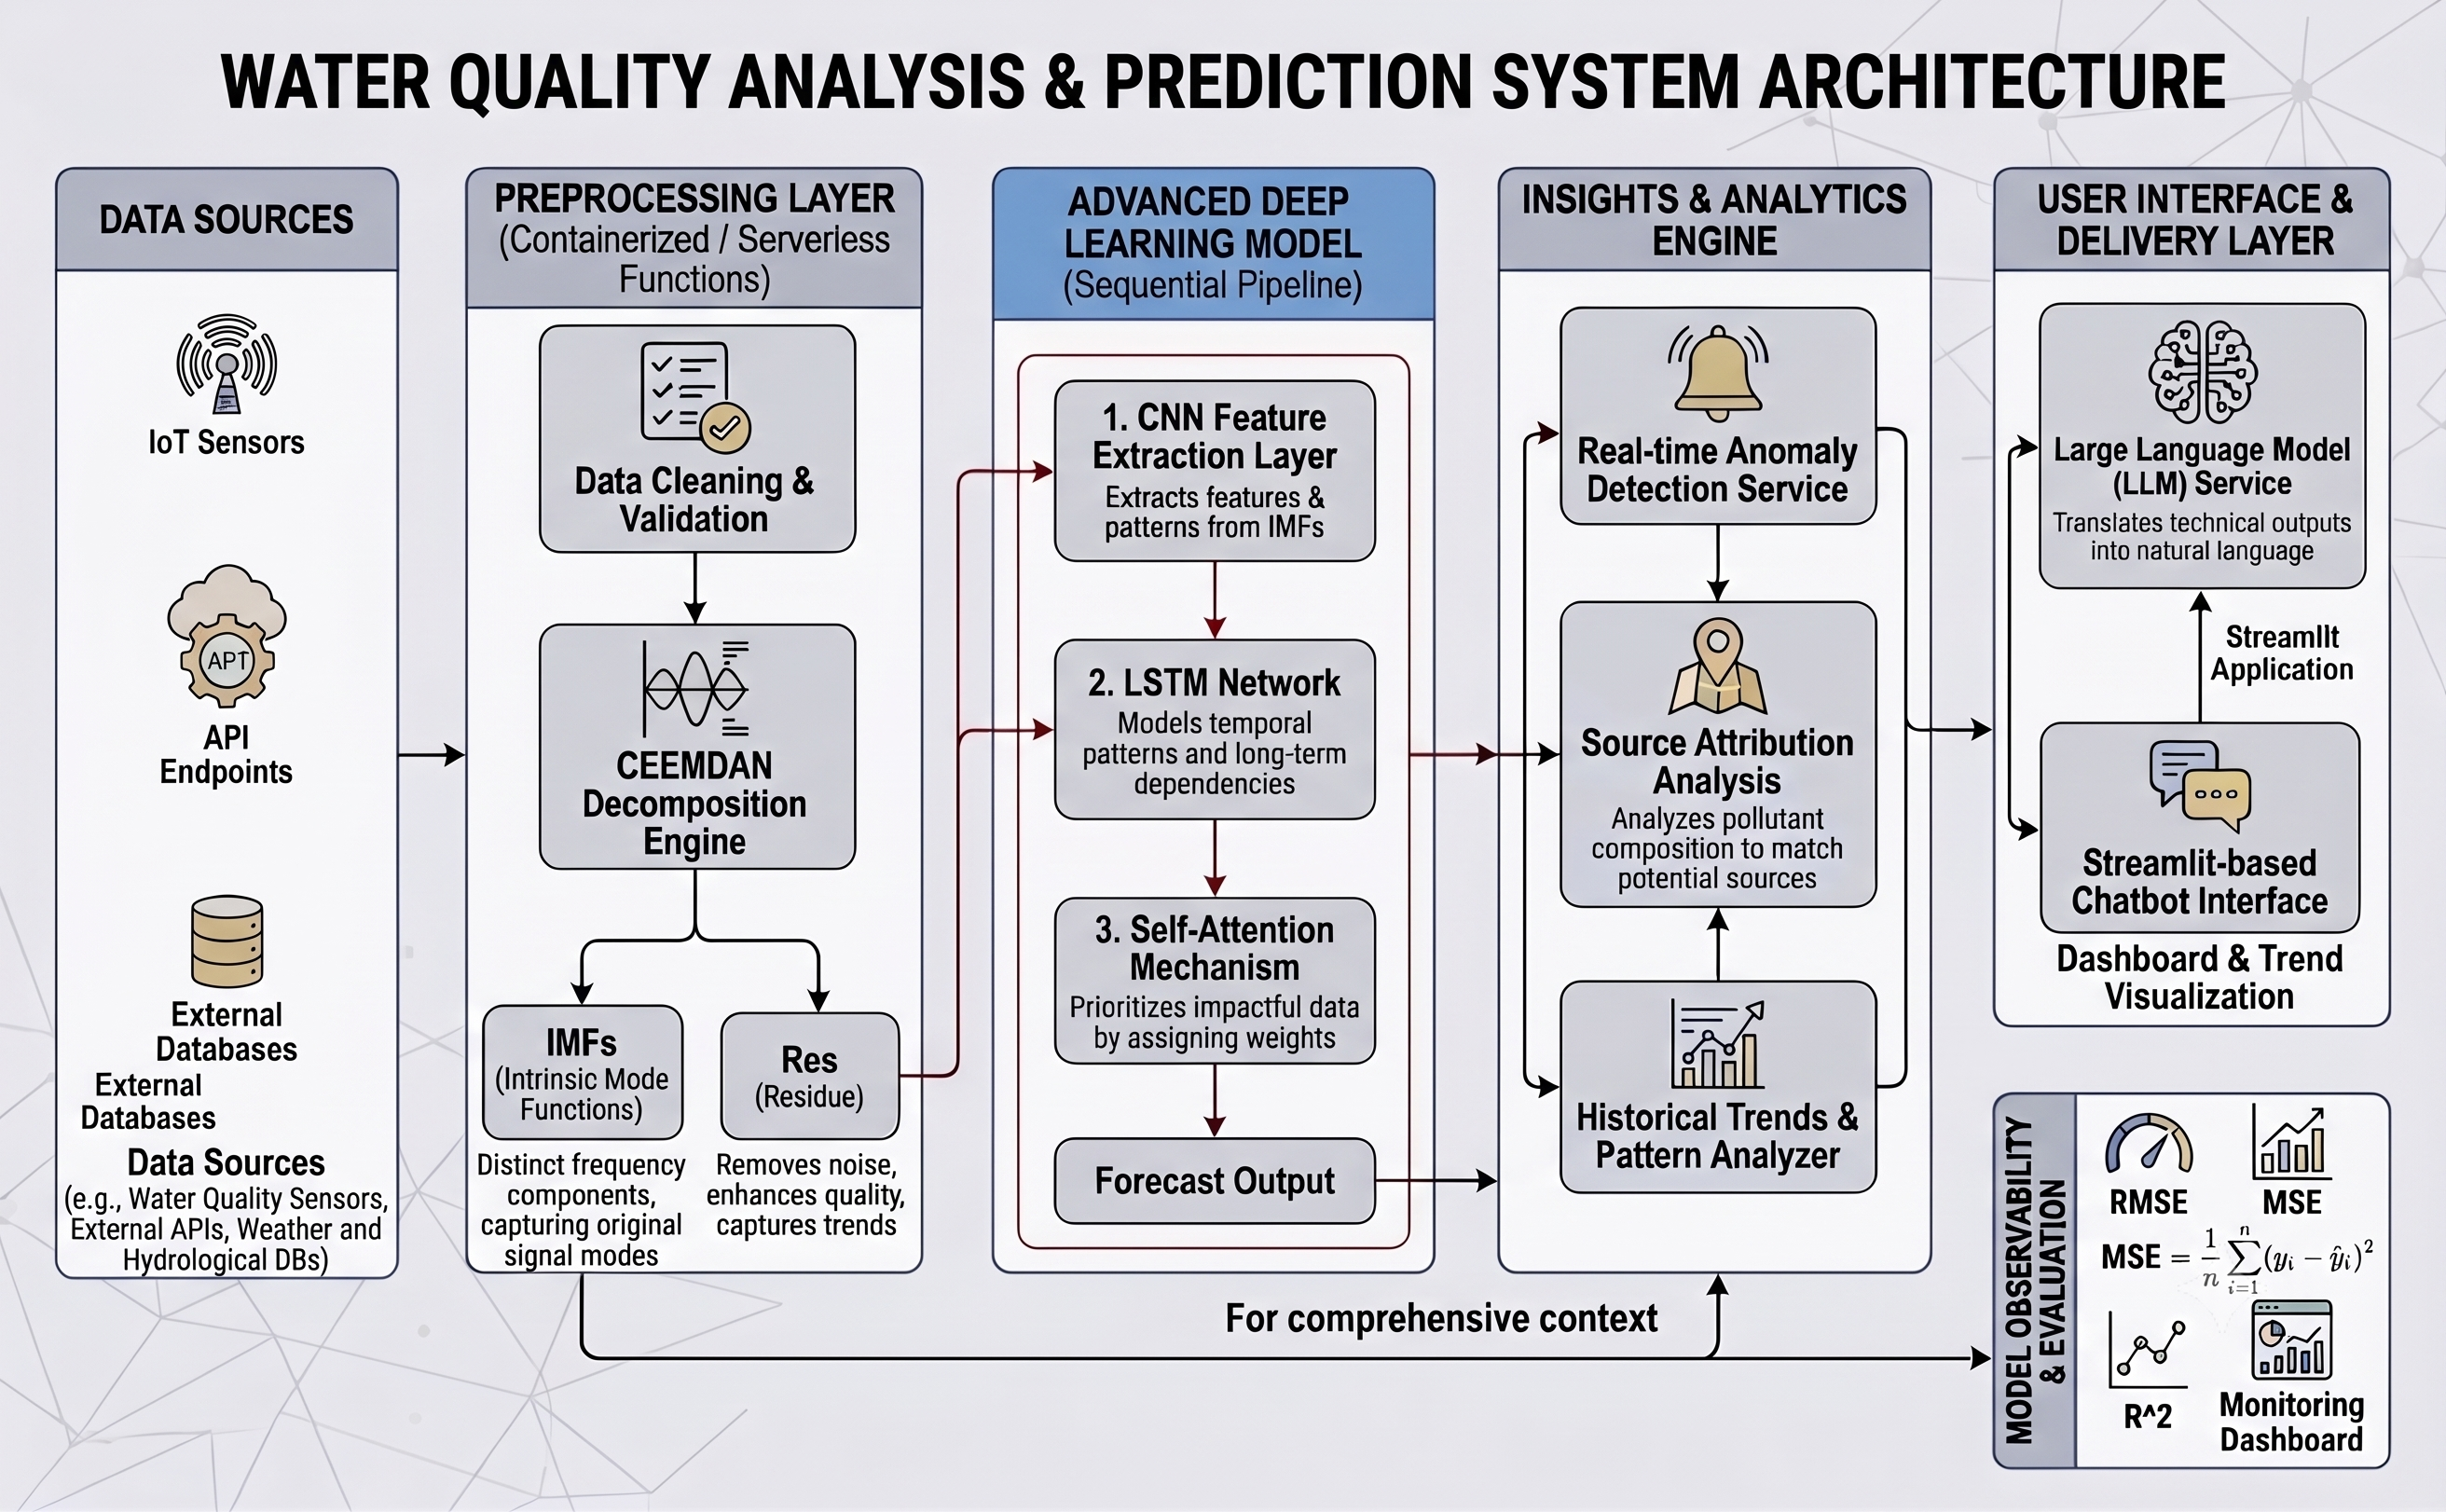
\includegraphics[width=0.94\textheight]{fig_architecture.png}
\caption{Water quality analysis and prediction system architecture. Readings
enter from sensors, APIs and external hydrological databases; the preprocessing
layer cleans them and applies CEEMDAN, emitting intrinsic mode functions and a
residual. The deep learning pipeline applies CNN feature extraction, an LSTM
for temporal dependency and self-attention for weighting, producing the
forecast. The insights engine performs anomaly detection, source attribution
and trend analysis, feeding an LLM service and Streamlit chatbot in the
delivery layer. Preprocessed signals are also routed directly to the analytics
engine for context, and evaluation metrics feed a monitoring dashboard. The
diagram describes the target deployment; the evaluation reported in
Section~\ref{sec:results} uses an archival dataset rather than live sensor
ingest.}
\label{fig:arch}
\end{sidewaysfigure*}


\subsection{Data Acquisition and Preprocessing}

This layer ingests raw readings and applies CEEMDAN, which separates a
nonstationary signal into intrinsic mode functions (IMFs) and a residual, each
IMF capturing an oscillatory mode from high-frequency noise to low-frequency
trend:

\begin{equation}
X_{\text{param}}(t) = \sum_{k=1}^{N} \mathrm{IMF}_k(t) + r_N(t)
\end{equation}

CEEMDAN operates iteratively: white noise realisations are added to the current
residual, the first mode of each realisation is extracted by EMD, and their
ensemble mean is taken as the next IMF before being subtracted from the
residual. Averaging over realisations suppresses the mode-mixing that affects
plain EMD, while the adaptive noise schedule keeps the decomposition complete.
Algorithm~\ref{alg:ceemdan} states the procedure. Our implementation uses the
\texttt{EMD-signal} package with its default configuration: 100 noise
realisations per mode, noise amplitude $\epsilon = 0.005$, and termination when
the residual retains less than 5\% of the original power or spans a range below
1\% of the signal.

\begin{algorithm}[!t]
\SetAlgoLined
\DontPrintSemicolon
\KwIn{signal $x(t)$; trials $M=100$; noise amplitude $\epsilon$}
\KwOut{IMF set $\{c_k\}$ and residual $r_N$}
$r_0 \leftarrow x$; $k \leftarrow 0$\;
\While{stopping criteria not met}{
  $k \leftarrow k+1$\;
  \For{$m \leftarrow 1$ \KwTo $M$}{
    draw white noise $w_m$\;
    $d_m \leftarrow \mathrm{EMD}_1(r_{k-1} + \epsilon\,w_m)$ \tcp*{first mode}
  }
  $c_k \leftarrow \frac{1}{M}\sum_m d_m$ \tcp*{ensemble mean}
  $r_k \leftarrow r_{k-1} - c_k$\;
}
\Return $\{c_k\}$, $r_k$\;
\caption{CEEMDAN decomposition}
\label{alg:ceemdan}
\end{algorithm}

\begin{figure}[!t]
\centering
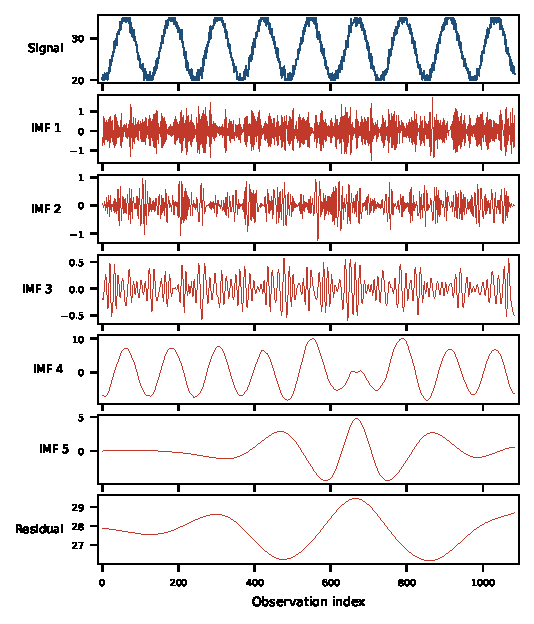
\includegraphics[width=0.86\columnwidth]{fig_imf.pdf}
\caption{CEEMDAN decomposition of the temperature series. The first modes carry
high-frequency measurement noise; later modes isolate the annual cycle, and the
residual captures the long-term trend. Eight modes were extracted for this
parameter.}
\label{fig:imf}
\end{figure}

Fig.~\ref{fig:imf} shows the decomposition applied to the temperature series.
The leading modes isolate high-frequency variation attributable to measurement
noise, intermediate modes recover the annual cycle, and the residual retains the
slow trend. This separation is what makes each component easier to model than
the composite signal.

Because CEEMDAN is adaptive, different parameters yield different IMF counts.
Temperature produced eight modes and the maximum across all nine parameters was
nine.
To obtain a fixed-width tensor the decomposition is zero-padded to the maximum
observed, $N=9$ for this dataset, so that each of the nine parameters
contributes nine channels and the network sees a constant 81-channel input.

\subsection{Hybrid Prediction Model}

The padded tensor passes through a stacked CNN--LSTM--attention network. The
1-D convolution extracts local morphological features; max pooling reduces
sequence length and suppresses jitter; the LSTM models
longer-range dependency; and self-attention~\cite{vaswani} performs learned
weighted pooling over the LSTM output. Given hidden states $\mathbf{x}$:

\begin{equation}
\mathbf{e} = \tanh(\mathbf{x}\mathbf{W} + \mathbf{b}), \quad
\boldsymbol{\alpha} = \mathrm{softmax}(\mathbf{e}), \quad
\mathbf{z} = \sum_t \mathbf{x}_t \odot \boldsymbol{\alpha}_t
\end{equation}

so each historical step's contribution is explicitly weighted, providing
interpretability absent from fixed pooling. Unlike scaled dot-product
attention, this formulation scores each time step against a single learned
projection rather than against every other step, which suits the short
30-step window and keeps the parameter count low.

Table~\ref{tab:shapes} traces the tensor through the network, with shapes and
parameter counts read from the saved model. The convolution dominates the
parameter budget because it must span all 81 input channels; the whole network
holds 41{,}625 trainable weights, small enough to train on 844 sequences
without severe overfitting, though the loss curve still requires early
stopping.

\begin{table}[!t]
\caption{Layer Functions, Tensor Shapes and Parameter Counts}
\label{tab:shapes}
\centering
\small
\setlength{\tabcolsep}{3.5pt}
\begin{tabular}{llrr}
\toprule
\textbf{Layer} & \textbf{Function} & \textbf{Output} & \textbf{Params} \\
\midrule
Input          & Padded IMF tensor      & $30\times81$ & 0 \\
Conv1D         & Local pattern extraction & $28\times64$ & 15{,}616 \\
MaxPooling1D   & Downsample, suppress jitter & $14\times64$ & 0 \\
LSTM           & Temporal dependency    & $14\times50$ & 23{,}000 \\
Self-attention & Weighted pooling       & $50$         & 2{,}550 \\
Dense          & Joint regression       & $9$          & 459 \\
\midrule
\multicolumn{3}{l}{\textbf{Total trainable parameters}} & \textbf{41{,}625} \\
\bottomrule
\end{tabular}
\end{table}

\subsection{Anomaly Detection and Attribution Layer}

Rather than predicting anomalies directly, the system monitors residuals.
During training the residual standard deviation $\sigma_f$ is recorded per
parameter $f$, and a reading is flagged when
$y_{\text{actual}} - y_{\text{pred}} > 3\sigma_f$. The test is deliberately
one-sided, flagging only anomalously high values and only for the six
pollution-indicative parameters, since a reading below prediction does not
indicate contamination.

Once an event is flagged, an attribution sub-module examines which parameters
moved together. Different industrial processes leave different signatures: a
joint rise in conductivity and total dissolved solids suggests saline or
chemical effluent, whereas elevated turbidity with nutrient species points
toward agricultural runoff or sediment mobilisation. Matching the observed
signature against a database of industrial discharge profiles, filtered by
geospatial proximity to the affected station, narrows the set of plausible
sources. Because proximity and compatibility are grounds for inclusion in a
shortlist rather than evidence of discharge, the output is presented as
candidate sources for investigation rather than as a determination.

\subsection{Service and User Application Layers}

A REST service exposes ingestion and retraining endpoints, with a scheduler
triggering quarterly retraining so the model tracks distributional drift as new
readings accumulate.

Above this sits the user application layer, which converts model output into a
form domain experts and the public can act on. A large language model
interprets predictions, alerts and attribution results, and answers natural
language questions against them, so that a query such as \emph{``river health
on 15 March 2024?''} returns a categorical assessment with its supporting
evidence rather than a vector of nine numbers. When an anomaly is active the
same channel raises the alert together with the shortlisted sources. A
Streamlit front-end hosts this conversation alongside trend visualisations,
letting users select a date range, trigger inference and toggle between raw
trends, flagged anomalies and the underlying decomposition.

This layer is what makes the residual-based detector usable in practice. A
$3\sigma$ exceedance on ammonia is not self-explanatory to a non-specialist,
whereas a statement that ammonia is anomalously high, that the shortlist
contains two facilities upstream, and that the reading is outside the range the
model was validated on, is directly actionable.

\begin{figure}[!t]
\centering
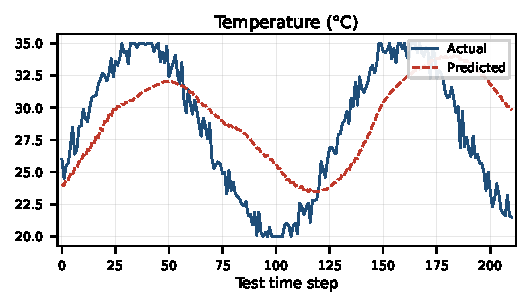
\includegraphics[width=\columnwidth]{fig_temperature.pdf}
\caption{Predicted versus actual temperature over the 211-step test horizon.
The annual cycle is tracked in correct phase, but peaks and troughs are
systematically under-shot.}
\label{fig:temp}
\end{figure}

\section{Implementation}

Implementation used Python 3 with TensorFlow and Keras, the \texttt{EMD-signal}
package for CEEMDAN, NumPy and Pandas, scikit-learn for scaling, and Flask for
the service layer.

\subsection{Dataset and Preprocessing}

The dataset comprises 1{,}085 multivariate observations from 1~January~2016 to
29~November~2024 at a median interval of three days, with no missing values
(Table~\ref{tab:data}). Turbidity is notably heavy-tailed, with a maximum of
149.8~NTU against a mean of 9.85~NTU, reflecting episodic runoff events.

The preprocessing sequence is summarised in Table~\ref{tab:prep}. Features and
targets are scaled independently to $[0,1]$ so predictions can be
inverse-transformed for thresholding. The feature scaler's column ordering is
persisted with the model; without this, IMF columns recomputed at inference can
be reordered relative to training, silently corrupting predictions.

\begin{table}[!t]
\caption{Dataset Summary (1{,}085 Observations, 2016--2024)}
\label{tab:data}
\centering
\small
\setlength{\tabcolsep}{4pt}
\begin{tabular}{lrrrr}
\toprule
\textbf{Parameter} & \textbf{Mean} & \textbf{Std} & \textbf{Min} & \textbf{Max} \\
\midrule
Temperature (\textdegree C)   & 27.58 & 5.27 & 20.00 & 35.0 \\
pH                            & 7.50 & 0.15 & 7.10 & 8.0 \\
Dissolved oxygen (mg/L)       & 8.99 & 1.39 & 7.00 & 11.0 \\
Conductivity ($\mu$S/cm)      & 448.22 & 51.83 & 293.10 & 607.4 \\
Turbidity (NTU)               & 9.85 & 17.84 & 2.00 & 149.8 \\
TDS (mg/L)                    & 290.88 & 34.90 & 189.90 & 407.1 \\
Ammonia (mg/L)                & 0.149 & 0.092 & 0.05 & 0.5 \\
Nitrates (mg/L)               & 1.482 & 0.891 & 0.50 & 4.0 \\
Phosphates (mg/L)             & 0.069 & 0.048 & 0.02 & 0.3 \\
\bottomrule
\end{tabular}
\end{table}

\begin{table}[!t]
\caption{Preprocessing Pipeline}
\label{tab:prep}
\centering
\small
\setlength{\tabcolsep}{3pt}
\begin{tabular}{L{2.1cm}L{2.3cm}L{2.9cm}}
\toprule
\textbf{Step} & \textbf{Purpose} & \textbf{Method} \\
\midrule
Type coercion & Numeric dtype & \texttt{to\_numeric}, coerced \\
Decomposition & Separate trend, noise & CEEMDAN, 100 trials \\
IMF padding & Uniform tensor width & Zero-pad to $N_{\max}=9$ \\
Normalisation & Consistent scale & Min--max to $[0,1]$ \\
Windowing & Supervised pairs & 30-step sliding window \\
Splitting & Prevent leakage & Chronological 80/20 \\
\bottomrule
\end{tabular}
\end{table}

\subsection{Sequence Construction and Configuration}

A sliding window of 30 steps predicts the observation at step 31, giving
1{,}055 sequences split chronologically (never randomly, which would leak
future information) into 844 training and 211 test. Each input has shape
$30 \times 81$, since nine parameters each contribute nine padded IMF channels.
Table~\ref{tab:arch} lists the configuration; all nine parameters are output
jointly from one dense layer, so a single network is trained.

\begin{table}[!t]
\caption{Model Architecture and Hyperparameters}
\label{tab:arch}
\centering
\small
\begin{tabular}{ll}
\toprule
\textbf{Component} & \textbf{Configuration} \\
\midrule
Input shape        & $30 \times 81$ \\
Conv1D             & 64 filters, kernel 3, ReLU \\
MaxPooling1D       & pool size 2 \\
LSTM               & 50 units, ReLU, return sequences \\
Self-attention     & tanh scoring, softmax weighting \\
Dense output       & 9 units (one per parameter) \\
Loss / optimiser   & MSE / Adam \\
Epochs / batch     & 50 / 32 \\
\bottomrule
\end{tabular}
\end{table}

At inference the service recomputes CEEMDAN over a trailing 200-observation
window, reorders columns to the persisted order, and predicts from the final 30
steps. This keeps inference cost stable as the archive grows, though it
introduces an inconsistency discussed in Section~\ref{sec:diag}.

\subsection{Interface and Chatbot Integration}

The front-end is built in Streamlit, chosen for rapid iteration and native
support for interactive plots. Table~\ref{tab:ui} traces the three principal
user actions through to the backend operation each triggers. Selecting a
forecast date prepares the corresponding 30-step window; running an analysis
invokes CEEMDAN over the trailing window followed by model inference; and
asking the chatbot for an explanation routes the current prediction, its
residual context and any active alerts to the language model for
interpretation.

\begin{table}[!t]
\caption{User Actions and Corresponding Backend Operations}
\label{tab:ui}
\centering
\small
\setlength{\tabcolsep}{3pt}
\begin{tabular}{L{1.75cm}L{2.2cm}L{3.0cm}}
\toprule
\textbf{User action} & \textbf{Backend} & \textbf{Output} \\
\midrule
Select forecast date & Prepare 30-step window & Window confirmation \\
Run analysis & CEEMDAN $\rightarrow$ inference & Predicted values, plots \\
Ask ``why?'' & LLM over prediction context & Natural-language summary \\
Export & Serialise results & CSV or PDF download \\
\bottomrule
\end{tabular}
\end{table}

Two design choices in this layer follow directly from the findings reported in
Section~\ref{sec:results}. First, because the model was trained and validated
for single-step prediction, requests beyond that horizon carry an explicit
uncertainty note rather than being silently extrapolated. Second, because the
analysis in Section~\ref{sec:results}-B shows the predictions to be strongly
damped in amplitude, the interface presents forecasts alongside the observed
historical range for the same parameter, so a user can see that a prediction
sitting near the seasonal mean reflects model conservatism rather than a
genuine expectation of stable conditions. Presenting a damped point forecast
without that context would overstate its confidence.

\section{Results and Performance Analysis}
\label{sec:results}

Evaluation uses the held-out final 211 sequences, inverse-transformed to
physical units before scoring. We report MAE, RMSE and $R^2$ against two
baselines: \emph{persistence}, the appropriate reference for a short-horizon
forecaster, and \emph{train mean}, which establishes the $R^2=0$
line~\cite{hyndman}.

\begin{table}[!t]
\caption{Test-Set Performance Against Baselines (211 Sequences)}
\label{tab:results}
\centering
\small
\setlength{\tabcolsep}{3.5pt}
\begin{tabular}{lrrrrr}
\toprule
& \multicolumn{2}{c}{\textbf{MAE}} & \multicolumn{2}{c}{\textbf{RMSE}} & \\
\cmidrule(lr){2-3}\cmidrule(lr){4-5}
\textbf{Parameter} & \textbf{Model} & \textbf{Persist.} & \textbf{Model} & \textbf{Persist.} & \textbf{$R^2$} \\
\midrule
Temperature      & 3.655 & \textbf{0.816} & 4.196 & 1.052 & 0.296 \\
pH               & \textbf{0.135} & 0.181 & 0.169 & 0.228 & $-0.173$ \\
Dissolved oxygen & 1.093 & \textbf{0.331} & 1.362 & 0.455 & $-0.040$ \\
Conductivity     & \textbf{42.00} & 60.08 & 52.69 & 72.79 & $-0.050$ \\
Turbidity        & \textbf{6.948} & 8.044 & 13.450 & 18.543 & $-0.128$ \\
TDS              & \textbf{28.21} & 42.43 & 35.47 & 51.00 & $-0.011$ \\
Ammonia          & \textbf{0.071} & 0.082 & 0.088 & 0.116 & $-0.141$ \\
Nitrates         & \textbf{0.793} & 1.034 & 1.053 & 1.378 & $-0.075$ \\
Phosphates       & \textbf{0.040} & 0.050 & 0.050 & 0.070 & $-0.038$ \\
\bottomrule
\end{tabular}
\end{table}

The model reduces MAE against persistence on seven of nine parameters, with
largest gains on TDS (33.5\%), conductivity (30.1\%) and nitrates (23.3\%), and
improves RMSE on those same seven, indicating the gain is not purely an
artefact of outlier handling.

\subsection{Trend Capture Versus Point Accuracy}

The accuracy target set at the outset was not met: eight of nine parameters
have $R^2 \leq 0$, so on a squared-error basis the model does not improve on
predicting the training mean. Reporting this plainly matters, since much of the
surveyed literature omits such baselines~\cite{pandya,rahu}.

That headline figure, however, conflates two questions: whether the model knows
\emph{when} a parameter rises and falls, and \emph{how far}. Because $R^2$
penalises both jointly, a predictor with correct phase but compressed amplitude
scores almost as harshly as one with no skill. We therefore report Pearson
correlation $r$, which is scale-invariant and so measures trend agreement
alone, alongside the variance ratio $\sigma_{\text{pred}}/\sigma_{\text{act}}$
in Table~\ref{tab:trend}.

\begin{table}[!t]
\caption{Trend Agreement and Amplitude Ratio}
\label{tab:trend}
\centering
\small
\begin{tabular}{lrrr}
\toprule
\textbf{Parameter} & \textbf{Pearson $r$} & \textbf{$\sigma_{\text{pred}}/\sigma_{\text{act}}$} & \textbf{$R^2$} \\
\midrule
Temperature      & \textbf{0.562} & 0.653 & 0.296 \\
Dissolved oxygen & \textbf{0.481} & 0.727 & $-0.040$ \\
\midrule
Conductivity     & 0.034 & 0.209 & $-0.050$ \\
TDS              & 0.066 & 0.190 & $-0.011$ \\
Turbidity        & 0.005 & 0.360 & $-0.128$ \\
pH               & $-0.010$ & 0.276 & $-0.173$ \\
Ammonia          & $-0.031$ & 0.166 & $-0.141$ \\
Nitrates         & $-0.061$ & 0.074 & $-0.075$ \\
Phosphates       & 0.008 & 0.140 & $-0.038$ \\
\bottomrule
\end{tabular}
\end{table}

The outcome is sharply bimodal. For the two seasonally driven parameters the
model achieves moderate positive correlation ($r=0.562$ for temperature,
$0.481$ for dissolved oxygen) while reproducing 65--73\% of observed variance.
Temporal structure is therefore genuinely learned: Fig.~\ref{fig:temp} shows
predicted temperature following the annual cycle in correct phase, and the
dissolved oxygen panel of Fig.~\ref{fig:grid} tracks the mid-series depression
and recovery. What the model gets wrong is magnitude, under-shooting peaks and
troughs. This is the signature of a regressor trained under squared error on a
partly unpredictable target, where shrinking toward the conditional mean
minimises loss.

For the remaining seven parameters correlation is statistically
indistinguishable from zero ($|r| < 0.07$) and the variance ratio falls to
0.07--0.36, so the output is effectively constant. These are precisely the
parameters governed by episodic external forcing (runoff, discharge events,
sediment mobilisation) rather than the smooth seasonal cycle. Their behaviour
is not encoded in their own recent history, so no purely autoregressive model,
however expressive, can recover it from the inputs supplied.

\begin{figure}[!t]
\centering
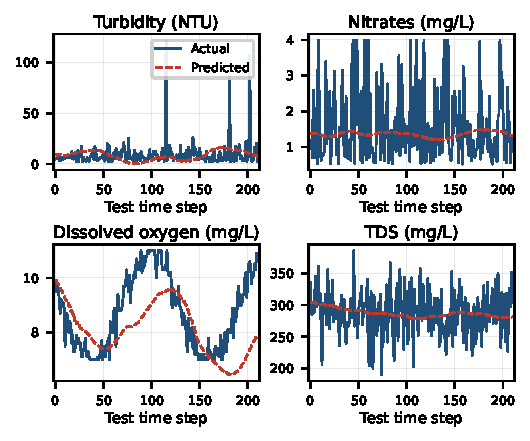
\includegraphics[width=\columnwidth]{fig_grid.pdf}
\caption{Predicted (dashed) versus actual (solid) traces. Dissolved oxygen
shows correct phase with damped amplitude; the remaining panels show
near-constant output, reflecting parameters driven by external forcing absent
from the input.}
\label{fig:grid}
\end{figure}

\begin{figure}[!t]
\centering
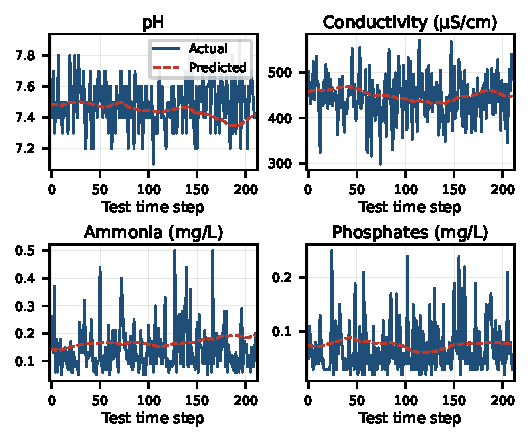
\includegraphics[width=\columnwidth]{fig_grid2.pdf}
\caption{Predicted (dashed) versus actual (solid) traces for the remaining four
parameters. All show the near-constant output characteristic of a model
predicting close to the conditional mean.}
\label{fig:grid2}
\end{figure}

Fig.~\ref{fig:grid2} completes the picture for the four parameters not shown
earlier. pH illustrates the central point most sharply: its observed range is
narrow (7.10--7.90 across the test set, standard deviation 0.15), so a
near-constant prediction achieves an MAE of only 0.135, under 2\% of the mean
value, while explaining none of the variance ($R^2 = -0.173$). A reader shown
the error alone would judge this the model's strongest result rather than one
of its weakest.

Conductivity and TDS are physically coupled through ionic content, and in the
observations they correlate at $r = 0.956$. The model's predictions for the two
correlate at only $0.679$, so the network has not reproduced the strongest
inter-parameter relationship in the data despite predicting both from a shared
representation through a single dense layer. Capturing such coupling was part
of the motivation for a joint output, and the gap suggests the shared layer is
too thin to encode it.

\subsection{Why Persistence Wins Where It Does}

The split in Table~\ref{tab:results} between parameters where persistence beats
the model and those where it fails badly is not arbitrary. It is predicted
almost exactly by a single property of the raw series: the lag-1
autocorrelation, shown in Fig.~\ref{fig:acf} and tabulated in
Table~\ref{tab:acf}.

\begin{figure}[!t]
\centering
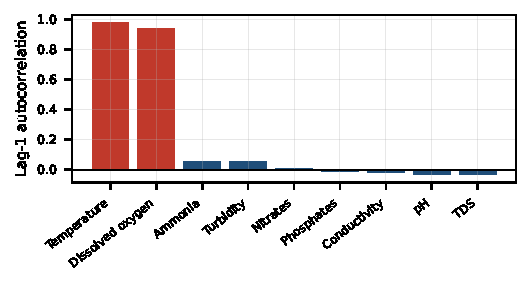
\includegraphics[width=\columnwidth]{fig_acf.pdf}
\caption{Lag-1 autocorrelation of each raw series. Only temperature and
dissolved oxygen (dark red) retain substantial correlation at the three-day
sampling interval; the remaining seven are indistinguishable from white noise
at this lag.}
\label{fig:acf}
\end{figure}

\begin{table}[!t]
\caption{Autocorrelation, Damping Slope and Skill}
\label{tab:acf}
\centering
\small
\setlength{\tabcolsep}{4pt}
\begin{tabular}{lrrr}
\toprule
\textbf{Parameter} & \textbf{Lag-1 ACF} & \textbf{Slope $b$} & \textbf{$R^2$} \\
\midrule
Temperature      & \textbf{0.980} & 0.367 & 0.296 \\
Dissolved oxygen & \textbf{0.943} & 0.350 & $-0.040$ \\
\midrule
Turbidity        & 0.054 & 0.002 & $-0.128$ \\
Ammonia          & 0.054 & $-0.005$ & $-0.141$ \\
Nitrates         & 0.008 & $-0.005$ & $-0.075$ \\
Phosphates       & $-0.009$ & 0.001 & $-0.038$ \\
Conductivity     & $-0.016$ & 0.007 & $-0.050$ \\
pH               & $-0.031$ & $-0.003$ & $-0.173$ \\
TDS              & $-0.034$ & 0.013 & $-0.011$ \\
\bottomrule
\end{tabular}
\end{table}

Temperature and dissolved oxygen have lag-1 autocorrelations of 0.980 and
0.943: at a three-day interval, yesterday's reading is almost the whole answer,
which is precisely why persistence attains $R^2 = 0.956$ on temperature and
$0.884$ on dissolved oxygen. Any model must clear a very high bar on these two,
and ours does not.

The other seven parameters have $|\text{ACF}| \leq 0.054$, statistically
indistinguishable from white noise at this lag. Their three-day-ahead values
are effectively unpredictable from their own recent history, so persistence
scores $R^2 \approx -1$ by echoing noise, and any method that shrinks toward
the mean beats it. Our model's apparent advantage on seven of nine parameters
is therefore largely an artefact of the baseline being pathological on exactly
those channels, not evidence of learned dynamics. This is a
sobering reading of our own headline result, and we state it explicitly
because the earlier comparison invites the opposite conclusion.

\begin{figure}[!t]
\centering
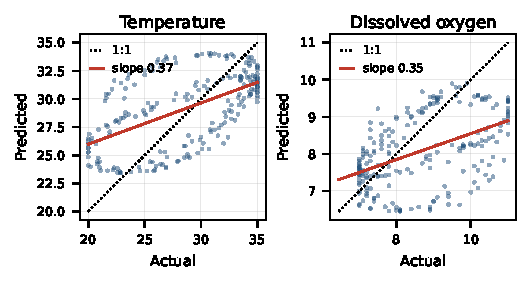
\includegraphics[width=\columnwidth]{fig_scatter.pdf}
\caption{Predicted against actual values for the two learnable parameters.
The fitted slope (solid) falls well below the 1:1 line (dotted), quantifying
the amplitude damping: the model spans roughly a third of the observed range.}
\label{fig:scatter}
\end{figure}

Column three of Table~\ref{tab:acf} quantifies the damping directly. Regressing
predicted on actual values gives a slope $b$ that would equal one for a
calibrated predictor. Temperature attains $b = 0.367$ and dissolved oxygen
$b = 0.350$, so both reproduce roughly a third of the observed dynamic range,
visible as the flattened point cloud in Fig.~\ref{fig:scatter}. For the other
seven, $|b| \leq 0.013$: the predictions are essentially flat, confirming that
the near-zero correlations of Table~\ref{tab:trend} reflect an absence of
signal rather than a phase error.

Taken together, the two columns give a compact diagnostic. Lag-1
autocorrelation says whether a parameter is learnable from its own history at
all; the damping slope says how much of the learnable amplitude the model
actually recovered. Reporting both would let readers of the wider literature
distinguish genuine dynamic modelling from mean reversion, which aggregate
error metrics cannot do.

\subsection{Diagnosis and Anomaly Detection}
\label{sec:diag}

Two implementation defects plausibly contribute. First, \textbf{decomposition
leakage}: CEEMDAN is applied to the whole series before the chronological
split, so each IMF is computed from the full record and training inputs contain
test-period information. Second, a \textbf{train/inference mismatch}: training
decomposes the full series whereas inference uses a trailing window, and IMFs
over different support are not comparable. Zero-padding to $N_{\max}=9$ and an
unweighted MSE across jointly scaled outputs further dilute the signal.

Residual standard deviations recorded during training form the detection
baseline for the six pollution-indicative parameters, listed in
Table~\ref{tab:sigma}. Turbidity, ammonia, nitrates and phosphates are excluded
from the temperature, pH and dissolved oxygen set because only they indicate
contamination when elevated; a reading below prediction carries no such
meaning, so the test is deliberately one-sided.

\begin{table}[!t]
\caption{Residual Baselines and $3\sigma$ Alert Thresholds}
\label{tab:sigma}
\centering
\small
\begin{tabular}{lrrr}
\toprule
\textbf{Parameter} & \textbf{$\sigma$} & \textbf{$3\sigma$} & \textbf{\% of mean} \\
\midrule
Conductivity ($\mu$S/cm) & 52.18 & 156.53 & 34.9 \\
Turbidity (NTU)          & 13.43 & 40.30  & 409.3 \\
TDS (mg/L)               & 35.47 & 106.40 & 36.6 \\
Ammonia (mg/L)           & 0.084 & 0.253  & 169.4 \\
Nitrates (mg/L)          & 1.023 & 3.070  & 207.3 \\
Phosphates (mg/L)        & 0.049 & 0.147  & 213.6 \\
\bottomrule
\end{tabular}
\end{table}

\begin{figure}[!t]
\centering
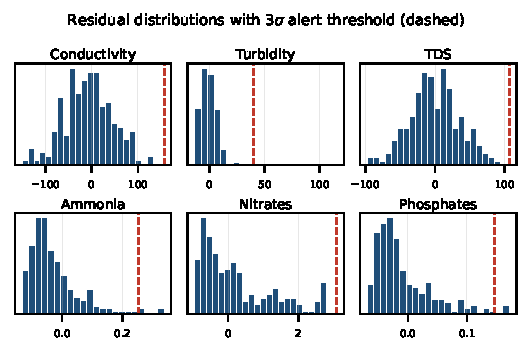
\includegraphics[width=\columnwidth]{fig_residuals.pdf}
\caption{Residual distributions for the six monitored parameters, with the
$3\sigma$ alert threshold marked. Heavy right tails on turbidity and the
nutrient species place the threshold far above the bulk of the distribution.}
\label{fig:residuals}
\end{figure}

The final column of Table~\ref{tab:sigma} exposes a practical limitation.
For conductivity and TDS the threshold sits at roughly a third of the mean
value, which is a plausible alerting level. For turbidity it is over four times the
mean, and for the three nutrient species between 1.7 and 2.1 times: an ammonia
excursion would have to reach 0.25~mg/L above prediction before firing, against
a mean of 0.149~mg/L. Fig.~\ref{fig:residuals} shows why. These parameters have heavy
right-tailed residual distributions, so their standard deviation is inflated by
the same rare events the detector is meant to catch. The system therefore
favours precision over recall, which suits an alerting context where false
alarms erode operator trust, but it will miss moderate contamination. A
quantile-based threshold estimated on a robust scale such as the median
absolute deviation would be better matched to these distributions than a
Gaussian $3\sigma$ rule.

\subsection{Limitations}

Three limitations bound the results. First, the evaluation covers a single
station and a single river, so spatial generalisability is untested; the
literature reviewed in Section~I-B identifies this as a recurring weakness and
our design does not escape it. Second, the model predicts one step ahead, and
because the sampling interval is three days the effective horizon is short.
Multi-horizon forecasting would require either recursive application, which
compounds the amplitude damping already observed, or a direct multi-output
formulation. Third, the anomaly layer has no ground truth: we can report the
thresholds it derives, but without confirmed pollution incidents we cannot
state a detection rate or false-alarm rate, and no claim about operational
performance should be inferred from its inclusion here.

\section{Conclusion}

This work presented a CEEMDAN--CNN--LSTM framework with self-attention for
multivariate river water quality prediction, coupled to a residual-based
anomaly detector and deployed with automated quarterly retraining. On a
1{,}085-observation record the model reduced both MAE and RMSE against
persistence on seven of nine parameters, by up to 33\%.

The point accuracy targeted at the outset was not reached, and we report that
directly. Separating trend agreement from amplitude, however, shows the
headline $R^2$ to be misleading as a summary of what was learned. On the
seasonally driven parameters the network tracks the observed trajectory in
correct phase while reproducing only 65--73\% of its variance: it has learned
\emph{when} these parameters move, but not \emph{how far}. On the seven
parameters governed by episodic external forcing no temporal structure is
recovered, the expected outcome for an autoregressive model whose inputs
contain no record of the driving events.

Both findings point the same way. Amplitude and event timing are set largely by
catchment conditions such as rainfall and runoff, land use, upstream discharge
and sediment transport. None of these is observable from a station's own
history, but all are carried by remotely sensed catchment
data~\cite{sagan,pahlevan}.

Beyond the architectural direction below, three implementation corrections
follow directly from Section~IV-C and should be made first, since each is a
defect rather than a design limit: fitting CEEMDAN on the training partition
alone, applying identical windowing at training and inference, and replacing
the shared zero-padded tensor with per-parameter decomposition heads. A
per-parameter loss weighting would additionally stop the high-variance
channels from dominating the gradient.

Future work should then pair this temporal expert with a \emph{spatial
expert} rather than keep enlarging the sequence model: spectral indices derived
from multispectral imagery over each catchment, reduced to a compact feature
subset by evolutionary selection and regressed with a random forest suited to
the small-sample, high-dimensional regime. An attention gate learning
per-sample weights $w_t$ and $w_s$ would then arbitrate between them, deferring
to the temporal stream for the seasonal parameters it already tracks and to
spatial evidence for the runoff-driven parameters where it is uninformative.
Establishing that the temporal stream captures trend reliably is what makes
this division of labour viable. The defects in Section~\ref{sec:diag} should be
corrected alongside it, since amplitude damping will otherwise limit the gain
from fusion, and extending across multiple stations so neighbouring sites
inform one another~\cite{yan} remains a natural longer-term step.

\begin{thebibliography}{00}

\bibitem{zhu} Q. Zhu, X. Yu, L. Zhao, and L. Xu, ``A hybrid deep learning
model for water quality prediction,'' \emph{Journal of Water Quality Analysis},
Jun. 2025.

\bibitem{yan} M. Yan and Z. Wang, ``Water quality prediction method based
on reinforcement learning graph neural network,'' \emph{Journal of
Environmental Engineering}, Dec. 2024.

\bibitem{shu} P. Shu et al., ``Deep learning-based super-resolution of
remote sensing images for enhanced groundwater quality assessment and
environmental monitoring in urban areas,'' \emph{Environmental Monitoring and
Remote Sensing Letters}, Mar. 2025.

\bibitem{sudriani} Y. Sudriani, V. Sebesty\'en, and J. Abonyi,
``Surface water monitoring systems---the importance of integrating information
sources for sustainable watershed management,'' \emph{Journal of Hydrology and
Water Resources}, Mar. 2023.

\bibitem{pandya} J. K. Pandya, S. S. Khandelwal, R. K. Tipu, and K. S.
Pandya, ``Advancing water quality management: an integrated approach using
ensemble machine learning and real-time interactive visualization,''
\emph{International Journal of Water Informatics}, May 2025.

\bibitem{rahu} M. A. Rahu et al., ``Toward design of IoT and machine
learning-enabled frameworks for analysis and prediction of water quality,''
\emph{International Journal of Smart Water Systems}, Sep. 2023.

\bibitem{vaswani} A. Vaswani et al., ``Attention is all you need,'' in
\emph{Proc. NeurIPS}, 2017, pp. 5998--6008.

\bibitem{hyndman} R. J. Hyndman and G. Athanasopoulos, \emph{Forecasting:
Principles and Practice}, 3rd ed. Melbourne: OTexts, 2021.

\bibitem{sagan} V. Sagan et al., ``Monitoring inland water quality using
remote sensing: potential and limitations of spectral indices, bio-optical
simulations, machine learning, and cloud computing,'' \emph{Earth-Science
Reviews}, vol. 205, art. 103187, 2020.

\bibitem{pahlevan} N. Pahlevan et al., ``Seamless retrievals of chlorophyll-a
from Sentinel-2 (MSI) and Sentinel-3 (OLCI) in inland and coastal waters,''
\emph{Remote Sensing of Environment}, vol. 240, art. 111604, 2020.

\end{thebibliography}

\end{document}
